\chapter{芭堤酒店实施}
%\label{cha:shigongtu}

\section{机房}

机房实景如图~\ref{fig:back}所示。我们的ROS放在机架最上面,负责整个酒店的用户身份认证功能,
用下来性能还不错。eth0口连接酒店的外网,eth1连接酒店的总交换机,总交换机连接每层楼的交换机,
每层楼的终端都要经过ROS路由器的认证才能够上网。

\begin{figure}[h]
  \centering
    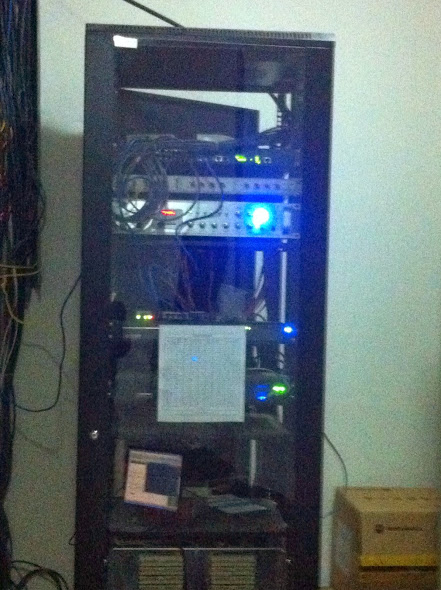
\includegraphics[width=.5\textwidth]{pic/back}
  \caption{机房}
  \label{fig:back}
\end{figure}

\section{前台}

前台实景如图~\ref{fig:front}所示。我们的树莓派+打印机+刷卡器,树莓派不需要人接触,直接放在
显示器后面。只要露出刷卡器和打印机给用户刷卡取纸就行了。刷卡器就是键盘旁边那个,打印机放在
旁边。
\begin{figure}[h]
  \centering
    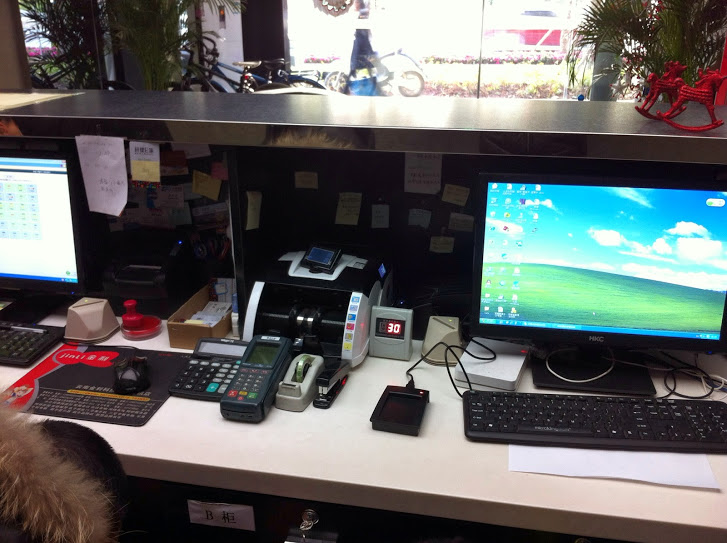
\includegraphics[width=.7\textwidth]{pic/front}
  \caption{前台}
  \label{fig:front}
\end{figure}

\section{Raspberry Pi}
%\label{sec:raspberry-pi}

图~\ref{fig:rasp}所示就是躲在角落里的树莓派,负责整个酒店的网络用户认证,总共有两个usb接口,
刷卡器接在树莓派的usb1口上,放在外面给人们刷卡,打印机接在树莓派usb2口上,放在外面打印用户
名密码,客户拿到纸条后安装纸条上的说明打开浏览器输入任意网址便会弹出带有badi酒店logo以及广
告的登录界面,然后输入用户名密码即可上网,客户离开的时候再去刷一次卡就自动下线了。另外使突
然断电也不影响酒店的网络使用,仅仅是暂时不能刷卡,只要恢复供电就又可以刷卡了。
\begin{figure}
  \centering
    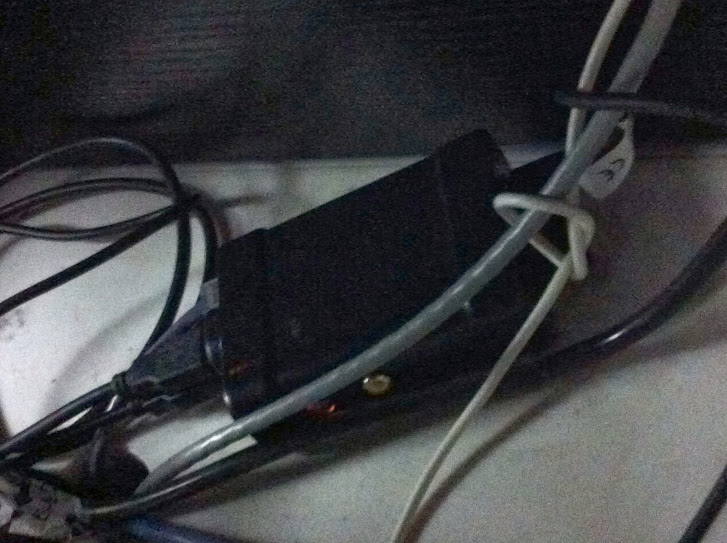
\includegraphics[width=.7\textwidth]{pic/rasp.JPG}
  \caption{树梅派}
  \label{fig:rasp}
\end{figure}

\section{实施心得}
通过在芭堤酒店的实施我得到了锻炼,我发现自己平时在学校只顾开发,从来没有和客户交流的概念,这样的话设
计出来的软件就会没有市场,我学会了要和客户交流,根据客户提出的一些建议改进
系统,比如客户提出希望操作简单方便,不要影响前台的电脑使用,我们就设想出了单独集成一套
Raspberry Pi的方案,简化了认证方式,使得工作人员不必手工去添加用户,同时不会影响前台电脑的使
用。随着使用时间的过去,根据反馈一点点改进,现在已经很稳定了,客户也很满意,产品也更成熟了。

%%% Local Variables: 
%%% mode: latex
%%% TeX-master: "../thesis"
%%% End: 
